\chapter{جمع‌بندی، نتیجه‌گیری و پیشنهادات برای کارهای آتی}
\section{جمع‌بندی و نتیجه‌گیری}
در این پروژه، سعی کردیم که یک رابط تحت وب برای ارائه خدمات \lr{IaaS} بر بستر \lr{VMWare Cloud Director} ارائه دهیم. در ابتدا با تحقیق و پیدا کردن نیازمندی‌ها، اقدام به طراحی معماری کلی سامانه و شناسایی ابزار‌ها و نیازمندی‌ها کردیم. سپس با تحقیق در مورد این نیازمندی‌ها و مزیت‌های هر مدل از پیاده‌سازی، به یک طراحی نهایی رسیدیم. برای طراحی این پیاده‌سازی از الگو‌های رایج توسعه نرم‌افزار تحت وب استفاده کردیم و به یک سامانه با قابلیت‌های قبول رسیدیم که به واسطه ساختار قطعه‌ای، قابلیت توسعه و تکمیل کردن به راحتی‌را دارد. سپس با ارزیابی‌های چندجانبه از صحت و توان عملکردی نرم‌افزار، پیش‌بینی تقریبی از اجرای این نرم‌افزار در سناریو‌های واقعی به دست آوردیم.

\section{پیشنهادات برای کارهای آتی}
این پروژه، قابلیت تکمیل و توسعه از ابعاد مختلفی را داراست. ساختار میکروسروییسی و وابستگی اندک سرویس‌ها به یکدیگر، امکان توسعه و تغییر در میکروسرویس‌ها را به صورت جداگانه می‌دهد. در ادامه برخی پیشنهادات برای تکمیل و توسعه را به صورت جامع توضیح می‌دهیم.

\subsection{تجزیه میکروسرویس ناظم}
عملکرد سرویس ناظم در حال حاضر، دربرگیرنده تنظیمات و تصمیمات کسب‌و‌کار از جمله مصرف کاربران و امور مالی است. در صورت نیاز و ظهور نیازمندی‌های کسب‌و‌کاری بیشتر، می‌توان قسمت ثبت مصرف و تصمیمات مالی را جداکرد. 

با این‌کار می‌توان مدل‌های مختلف پرداختی را پشتیبانی کرد. این جداسازی مزیت جداشدن منطق و محدودتر شدن فعالیت‌های میکروسرویس را به دنبال دارد. منتها سربار منابع مصرفی اضافی و افزایش تعداد درخواست‌ها در شبکه را نیز اضافه می‌کند.


\subsection{ارتباطات رخداد پایه}
در حال حاضر، تمام ارتباطات سامانه به صورت سنکرون و توسط درخواست‌های \lr{HTTP} انجام می‌شود. مزیت این روش سادگی پیاده‌سازی و دنبال کردن روند اجرای‌ دستورات است. منتها با افزایش تعداد درخواست‌ها و محدودیت‌های شبکه ، این مشکل پیش می‌آید که بازیابی وضعیت سیستم از خطا دشوارتر می‌شود. برای افزایش آستانه تحمل خطا در سرویس‌ها و امکان اضافه کردن تلاش مجدد\LTRfootnote{Retry}، می‌توان ارتباط سرویس‌ها را به صورت آسنکرون و به صورت رخداد پایه انجام داد. مزیت این‌کار بالابردن در دسترس بودن سیستم\LTRfootnote{Availability} می‌شود. برای پیاده‌سازی این مورد می‌توان از ابزارهای انتقال پیام نظیر \lr{Apache Kafka} یا راه‌حل‌های سبک‌تر نظیر \lr{NATS} استفاده کرد. 

نحوه پیاده‌سازی \lr{API} در میکروسرویس‌ها، امکان تغییر مکانیزم تعامل با بیرون را بسیار ساده کرده است. فقط کافی‌است که در پکیج‌های مربوطه، توابع مربوط به دریافت و ارسال اطلاعات را فارغ از نحوه پیاده‌سازی معرفی کنید. لایه‌های زیرین سرویس فقط نیازمند توابعی برای دریافت و ارسال اطلاعات هستند و وابستگی‌ای به نحوه دریافت و ارسال این اطلاعات ندارند.

معماری جدید سامانه در این حالت در شکل\ref{fig:30bird-cmq} مشخص شده است.

\begin{figure}
	\centering
	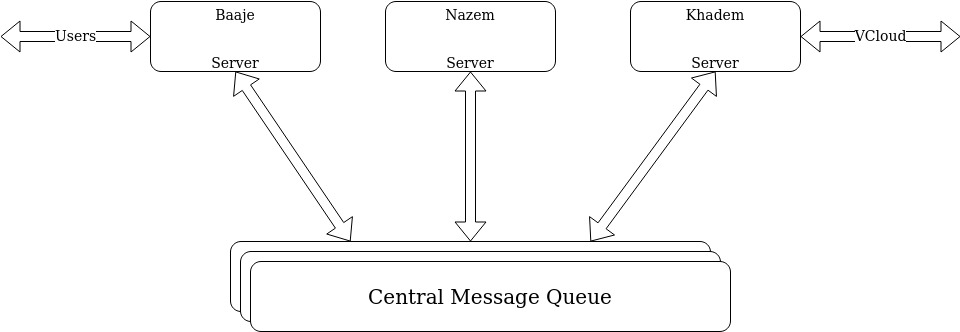
\includegraphics[scale=0.45]{figures/30bird-cmq.jpg}
	\caption{معماری سامانه در حالت آسنکرون}
	\label{fig:30bird-cmq}
\end{figure}


\subsection{نظارت و گزارش رخداد‌ها}
جهت بهبود وضعیت نظارت بر سامانه، می‌توان از داشبورد‌های گرافیکی ابزار گرافانا\LTRfootnote{Grafana} استفاده کرد. فقط کافیست که از اطلاعات متریک‌های سرور برای نمایش اطلاعات در قالب این داشبورد‌ها استفاده‌کرد.

مزیت دیگر استفاده از این ابزار، امکان تعریف هشدار\LTRfootnote{Alert} برای وضعیت‌های خاص و ناخواسته است. استفاده از این الگو، از روند‌های رایج در فرهنگ \lr{SRE}\LTRfootnote{Software Reliability Engineer} است. پیروی از این فرهنگ، بازیابی از فاجعه‌ها و ایرادات را بسیار سریع‌تر و آسان‌تر می‌کند.

اضافه کردن \lr{Telemetry} بسیار به درک و نظارت عملکرد میکروسرویس‌ها کمک می‌کند. ابزار پیشنهادی برای پیاده‌سازی این قابلیت، \lr{Jaeger} و کتاب‌خانه‌های \lr{OpenTelemetry} است.

\subsection{پشتیبانی از افزونه‌های \lr{VMWare Cloud Director}}
برخی از قابلیت‌های ابزار \lr{Cloud Director} در قالب افزونه‌ها ارائه شده که به صورت پیش‌فرض فعال نیستند و نیازمند تغییراتی در تنظیمات هستند. با فعال سازی این افزونه‌ها می‌توان از امکانات بیشتری از این سرویس استفاده کرد. یکی از مثال‌های این افزونه‌ها، افزونه نظارت (\lr{Monitoring}) است که نیازمند راه‌اندازی یک پایگاه \lr{Cassandra} است. با تنظیم کردن و اضافه کردن این افزونه، امکان دریافت جزئیات مصرف منابع و گزارش گیری از آنها را مستقیما از سمت \lr{Cloud Director} پیدا می‌کنیم.

البته پیاده‌سازی این این امکانات در سمت سرویس خادم با چالش‌هایی همراه است. چرا که این جزئیات در بسته توسعه نرم‌افزار پیش‌فرض تعبیه نشده و نیازمند تعامل مستقیم و خام برنامه با رابط برنامه‌نویسی \lr{vCloud} است. البته این امر می‌تواند به سادگی و با تبدیل دستورات برنامه رابط کاربری تحت وب به دستورات \lr{cURL} و سپس تبدیل دستورات \lr{cURL} به درخواست‌های \lr{HTTP} در زبان \lr{Go} توسط برنامه \lr{Postman} انجام شود. توسعه‌دهنده کافی است درخواست‌های ساخته‌شده را به قالب توابع موجود \texttt{VCloudManager} در بسته \texttt{vcloud} در برنامه تبدیل کند.